\documentclass{article}

% content/resources/templates/preamble.tex
\usepackage[margin=0.6in]{geometry}
\author{Milav Dabgar}
\usepackage{amsmath,amssymb,amsthm}
\usepackage{booktabs}
\usepackage{multirow}
\usepackage{xcolor}
\usepackage{tcolorbox}
\tcbuselibrary{breakable,skins}
\usepackage[colorlinks=true,linkcolor=blue]{hyperref}
\usepackage{titlesec}
\usepackage{enumitem}
\usepackage{tikz}
\usepackage{pgfplots}
\usepackage{circuitikz}
\usepackage[version=4]{mhchem}
\usepackage{longtable}
\usepackage{array}
\usepackage{float}
\usepackage{caption}
\usepackage{listings}

\lstset{
  basicstyle=\small\ttfamily,
  breaklines=true,
  breakatwhitespace=false,
  postbreak=\mbox{\textcolor{red}{$\hookrightarrow$}\space},
  float=false,
  numbers=left,
  numberstyle=\tiny\color{gray},
  numbersep=10pt,
  xleftmargin=2em,
  keywordstyle=\color{blue},
  commentstyle=\color{green!60!black},
  stringstyle=\color{purple},
  backgroundcolor=\color{gray!5},
  showstringspaces=false,
  tabsize=2,
  captionpos=b,
  keepspaces=true,
  columns=flexible
}

\pgfplotsset{compat=1.18}
\usetikzlibrary{shapes,arrows,positioning,calc,patterns,decorations.pathmorphing,decorations.markings,arrows.meta}

% Color scheme
\definecolor{headcolor}{RGB}{0,102,204}
\definecolor{keycolor}{RGB}{220,20,60}
\definecolor{solutioncolor}{RGB}{34,139,34}
\definecolor{mnemoniccolor}{RGB}{148,0,211}
\definecolor{codecolor}{RGB}{0,0,100}

% Spacing
\setlength{\parskip}{3pt}
\setlist[itemize]{nosep}
\setlist[enumerate]{nosep}

% Title formatting
\titleformat{\section}{\Large\bfseries\color{headcolor}}{\thesection}{1em}{}
\titleformat{\subsection}{\large\bfseries\color{headcolor}}{\thesubsection}{1em}{}

% Pandoc tightlist compatibility
\providecommand{\tightlist}{%
  \setlength{\itemsep}{0pt}\setlength{\parskip}{0pt}}

% Pandoc longtable compatibility
\newcounter{none}
\def\thenone{}


% content/resources/templates/english-boxes.tex
% This file is currently empty - it exists to maintain consistency with the import structure.
% Add custom environments here if needed in the future.


% Custom commands for GTU solutions
% This file defines semantic commands for consistent formatting

% Question command with automatic formatting
\newcommand{\question}[2]{%
  \section*{Question #1}%
  \textbf{#2}%
}

% OR question variant
\newcommand{\questionor}[2]{%
  \section*{Question #1 OR}%
  \textbf{#2}%
}

% Proper table environment with caption
\newenvironment{answertable}[1]{%
  \begin{table}[htbp]
  \centering
  \caption{#1}
}{%
  \end{table}
}

% Proper figure environment for diagrams
\newenvironment{answerdiagram}[1]{%
  \begin{figure}[htbp]
  \centering
  \caption{#1}
}{%
  \end{figure}
}

% Semantic markup for key terms
\newcommand{\keyword}[1]{\textbf{#1}}
\newcommand{\code}[1]{\texttt{#1}}
\newcommand{\classname}[1]{\texttt{#1}}
\newcommand{\methodname}[1]{\texttt{#1}}

% Proper quotation marks
\newcommand{\mnemonic}[1]{``#1''}


\title{Mobile \& Wireless Communication (4351104) - Winter 2023 Solution}
\date{December 12, 2023}

\begin{document}
\maketitle

\questionmarks{1(a)}{3}{Draw \& Explain umbrella cell.}
\begin{solutionbox}
    \begin{center}
        \begin{tikzpicture}[gtu flow]
            \node[gtu block] (umbrella) {Umbrella Cell Tower \\ (Large Coverage)};
            \node[gtu block, below left=1.5cm and 1cm of umbrella] (micro1) {Micro Cell 1};
            \node[gtu block, below=1.5cm of umbrella] (micro2) {Micro Cell 2};
            \node[gtu block, below right=1.5cm and 1cm of umbrella] (micro3) {Micro Cell 3};
            
            \node[gtu block, below=1cm of micro1] (users1) {Users in \\ Dense Area};
            \node[gtu block, below=1cm of micro2] (users2) {Users in \\ Dense Area};
            \node[gtu block, below=1cm of micro3] (users3) {Users in \\ Dense Area};
            
            \draw[gtu arrow] (umbrella) -- (micro1);
            \draw[gtu arrow] (umbrella) -- (micro2);
            \draw[gtu arrow] (umbrella) -- (micro3);
            \draw[gtu arrow] (micro1) -- (users1);
            \draw[gtu arrow] (micro2) -- (users2);
            \draw[gtu arrow] (micro3) -- (users3);
        \end{tikzpicture}
    \end{center}

    \begin{itemize}
        \item \textbf{Umbrella Cell}: Large coverage cell overlaying smaller cells.
        \item \textbf{Purpose}: Handles overflow traffic from micro/pico cells.
        \item \textbf{Coverage}: Provides backup coverage for high-traffic areas.
    \end{itemize}
\end{solutionbox}
\begin{mnemonicbox}
    \mnemonic{Under My Big Umbrella}
\end{mnemonicbox}

\questionmarks{1(b)}{4}{Define full forms: (i) CCH (ii) TCH (iii) SCH (iv) BCCH}
\begin{solutionbox}
    \begin{tabulary}{\linewidth}{|L|L|L|}
        \hline
        \textbf{Acronym} & \textbf{Full Form} & \textbf{Function} \\
        \hline
        CCH & Control Channel & Carries control information \\
        \hline
        TCH & Traffic Channel & Carries voice/data traffic \\
        \hline
        SCH & Synchronization Channel & Provides timing sync \\
        \hline
        BCCH & Broadcast Control Channel & Broadcasts system info \\
        \hline
    \end{tabulary}
\end{solutionbox}
\begin{mnemonicbox}
    \mnemonic{Control Traffic Sync Broadcast}
\end{mnemonicbox}

\questionmarks{1(c)}{7}{What is cell? Explain different types of cells.}
\begin{solutionbox}
    \textbf{Cell} is the basic coverage area served by one base station in cellular communication.

    \begin{tabulary}{\linewidth}{|L|L|L|L|}
        \hline
        \textbf{Cell Type} & \textbf{Coverage} & \textbf{Power} & \textbf{Usage} \\
        \hline
        \textbf{Macro Cell} & 1-30 km & High & Rural areas \\
        \hline
        \textbf{Micro Cell} & 100m-2km & Medium & Urban areas \\
        \hline
        \textbf{Pico Cell} & 10-100m & Low & Indoor coverage \\
        \hline
        \textbf{Femto Cell} & 10-30m & Very Low & Home/office \\
        \hline
    \end{tabulary}

    \begin{center}
        \begin{tikzpicture}[gtu flow]
            \node[gtu block] (macro) {Macro Cell \\ (Large Area)};
            \node[gtu block, right=1cm of macro] (micro) {Micro Cell \\ (City Coverage)};
            \node[gtu block, right=1cm of micro] (pico) {Pico Cell \\ (Building)};
            \node[gtu block, right=1cm of pico] (femto) {Femto Cell \\ (Room)};
            
            \draw[gtu arrow] (macro) -- (micro);
            \draw[gtu arrow] (micro) -- (pico);
            \draw[gtu arrow] (pico) -- (femto);
        \end{tikzpicture}
    \end{center}

    \begin{itemize}
        \item \textbf{Function}: Each cell provides wireless service to mobile users.
        \item \textbf{Frequency Reuse}: Same frequencies used in non-adjacent cells.
        \item \textbf{Handoff}: Users move between cells seamlessly.
    \end{itemize}
\end{solutionbox}
\begin{mnemonicbox}
    \mnemonic{Many Mobile People Find coverage}
\end{mnemonicbox}

\questionmarks{1(c) OR}{7}{What is handoff? Explain soft and hard handoffs.}
\begin{solutionbox}
    \textbf{Handoff} is the process of transferring an ongoing call from one cell to another as mobile moves.

    \begin{tabulary}{\linewidth}{|L|L|L|}
        \hline
        \textbf{Feature} & \textbf{Hard Handoff} & \textbf{Soft Handoff} \\
        \hline
        \textbf{Connection} & Break-before-make & Make-before-break \\
        \hline
        \textbf{Channels} & One at a time & Multiple simultaneously \\
        \hline
        \textbf{Technology} & GSM, TDMA & CDMA \\
        \hline
        \textbf{Quality} & Brief interruption & Seamless transition \\
        \hline
    \end{tabulary}

    \begin{center}
        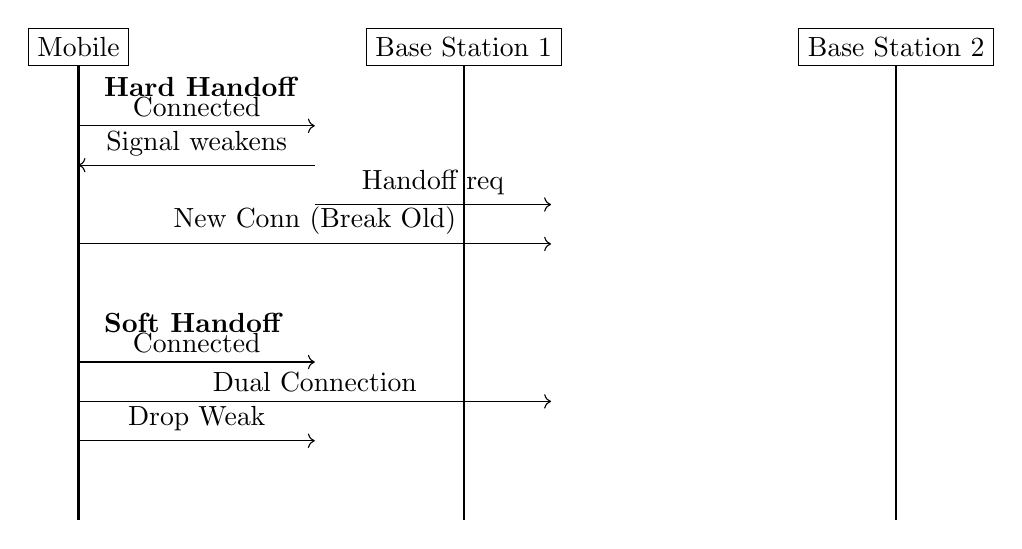
\begin{tikzpicture}[node distance=1.5cm, auto]
            % Actors
            \node[draw, rectangle] (M) {Mobile};
            \node[draw, rectangle, right=3cm of M] (BS1) {Base Station 1};
            \node[draw, rectangle, right=3cm of BS1] (BS2) {Base Station 2};

            % Timelines
            \draw[thick] (M) -- ++(0,-6);
            \draw[thick] (BS1) -- ++(0,-6);
            \draw[thick] (BS2) -- ++(0,-6);

            % Hard Handoff
            \node[anchor=west] at (0.2,-0.5) {\textbf{Hard Handoff}};
            \draw[->] (0,-1) -- (3,-1) node[midway, above] {Connected};
            \draw[<-] (0,-1.5) -- (3,-1.5) node[midway, above] {Signal weakens};
            \draw[->] (3,-2) -- (6,-2) node[midway, above] {Handoff req};
            \draw[->] (0,-2.5) -- (6,-2.5) node[midway, above] {New Conn (Break Old)};

            % Soft Handoff
            \node[anchor=west] at (0.2,-3.5) {\textbf{Soft Handoff}};
            \draw[->] (0,-4) -- (3,-4) node[midway, above] {Connected};
            \draw[->] (0,-4.5) -- (6,-4.5) node[midway, above] {Dual Connection};
            \draw[->] (0,-5) -- (3,-5) node[midway, above] {Drop Weak};
        \end{tikzpicture}
    \end{center}

    \begin{itemize}
        \item \textbf{Initiation}: Based on signal strength measurements.
        \item \textbf{MAHO}: Mobile Assisted Handoff improves decision accuracy.
    \end{itemize}
\end{solutionbox}
\begin{mnemonicbox}
    \mnemonic{Hard Hurts, Soft Smooth}
\end{mnemonicbox}

\questionmarks{2(a)}{3}{Define full forms: (i) SIM (ii) LTE (iii) WCDMA}
\begin{solutionbox}
    \begin{tabulary}{\linewidth}{|L|L|L|}
        \hline
        \textbf{Acronym} & \textbf{Full Form} & \textbf{Purpose} \\
        \hline
        SIM & Subscriber Identity Module & User authentication \\
        \hline
        LTE & Long Term Evolution & 4G technology \\
        \hline
        WCDMA & Wideband Code Division Multiple Access & 3G standard \\
        \hline
    \end{tabulary}
\end{solutionbox}
\begin{mnemonicbox}
    \mnemonic{Subscriber's Long Wideband connection}
\end{mnemonicbox}

\questionmarks{2(b)}{4}{Draw mobile handset block diagram.}
\begin{solutionbox}
    \begin{center}
        \begin{tikzpicture}[gtu flow]
            \node[gtu block] (antenna) {Antenna};
            \node[gtu block, below=1cm of antenna] (rf) {RF Section};
            \node[gtu block, below=1cm of rf] (baseband) {Baseband Processor};
            
            \node[gtu block, left=1cm of baseband] (display) {Display/Keypad};
            \node[gtu block, right=1cm of baseband] (audio) {Audio Section};
            \node[gtu block, below right=1cm and 0.1cm of baseband] (memory) {Memory};
            
            \node[gtu block, below left=1.5cm and 0.5cm of baseband] (power) {Power Management};
            \node[gtu block, left=1cm of power] (battery) {Battery};

            \draw[gtu arrow] (antenna) -- (rf);
            \draw[gtu arrow] (rf) -- (baseband);
            \draw[gtu arrow, <->] (baseband) -- (display);
            \draw[gtu arrow, <->] (baseband) -- (audio);
            \draw[gtu arrow, <->] (baseband) -- (memory);
            
            \draw[gtu arrow] (battery) -- (power);
            \draw[gtu arrow] (power) -| (rf);
            \draw[gtu arrow] (power) -| (baseband);
            \draw[gtu arrow] (power) -| (display);
        \end{tikzpicture}
    \end{center}

    \begin{itemize}
        \item \textbf{RF Section}: Transmits/receives radio signals.
        \item \textbf{Baseband}: Processes digital signals and protocols.
        \item \textbf{Audio}: Handles voice input/output.
        \item \textbf{Power Management}: Controls battery usage efficiently.
    \end{itemize}
\end{solutionbox}
\begin{mnemonicbox}
    \mnemonic{Radio Baseband Audio Power}
\end{mnemonicbox}

\questionmarks{2(c)}{7}{Explain GSM architecture with diagram.}
\begin{solutionbox}
    \begin{center}
        \begin{tikzpicture}[gtu flow]
            \node[gtu block] (ms) {MS};
            
            % BSS
            \node[gtu block, right=1.5cm of ms] (bts) {BTS};
            \node[gtu block, right=1cm of bts] (bsc) {BSC};
            \node[draw, dashed, fit=(bts)(bsc), label={[anchor=south]north:BSS}] (bss) {};
            
            % NSS
            \node[gtu block, right=1cm of bsc] (msc) {MSC};
            \node[gtu block, above=1cm of msc] (hlr) {HLR};
            \node[gtu block, below=1cm of msc] (vlr) {VLR};
            \node[gtu block, right=1cm of hlr] (auc) {AuC};
            \node[draw, dashed, fit=(msc)(hlr)(vlr)(auc), label={[anchor=south]north:NSS}] (nss) {};
            
            \node[gtu block, right=1.5cm of msc] (pstn) {PSTN};

            \draw[gtu arrow] (ms) -- (bts);
            \draw[gtu arrow] (bts) -- (bsc);
            \draw[gtu arrow] (bsc) -- (msc);
            \draw[gtu arrow] (msc) -- (pstn);
            \draw[gtu arrow] (msc) -- (hlr);
            \draw[gtu arrow] (msc) -- (vlr);
            \draw[gtu arrow] (hlr) -- (auc);
        \end{tikzpicture}
    \end{center}

    \begin{tabulary}{\linewidth}{|L|L|}
        \hline
        \textbf{Component} & \textbf{Function} \\
        \hline
        \textbf{MS} & Mobile Station (handset) \\
        \hline
        \textbf{BTS} & Base Transceiver Station \\
        \hline
        \textbf{BSC} & Base Station Controller \\
        \hline
        \textbf{MSC} & Mobile Switching Center \\
        \hline
        \textbf{HLR} & Home Location Register \\
        \hline
        \textbf{VLR} & Visitor Location Register \\
        \hline
    \end{tabulary}

    \begin{itemize}
        \item \textbf{BSS}: Base Station Subsystem handles radio interface.
        \item \textbf{NSS}: Network Switching Subsystem manages calls.
        \item \textbf{Authentication}: AuC verifies subscriber identity.
    \end{itemize}
\end{solutionbox}
\begin{mnemonicbox}
    \mnemonic{Mobile Base Network calls Home}
\end{mnemonicbox}

\questionmarks{2(a) OR}{3}{Define full forms: (i) RSSI (ii) MAHO (iii) NCHO}
\begin{solutionbox}
    \begin{tabulary}{\linewidth}{|L|L|L|}
        \hline
        \textbf{Acronym} & \textbf{Full Form} & \textbf{Function} \\
        \hline
        RSSI & Received Signal Strength Indicator & Signal quality measurement \\
        \hline
        MAHO & Mobile Assisted Handoff & Mobile helps handoff decision \\
        \hline
        NCHO & Network Controlled Handoff & Network decides handoff \\
        \hline
    \end{tabulary}
\end{solutionbox}
\begin{mnemonicbox}
    \mnemonic{Received Mobile Network signals}
\end{mnemonicbox}

\questionmarks{2(b) OR}{4}{Draw baseband section block diagram.}
\begin{solutionbox}
    \begin{center}
        \begin{tikzpicture}[gtu flow]
            \node[gtu block] (adc) {ADC/DAC};
            \node[gtu block, right=1cm of adc] (dsp) {DSP};
            \node[gtu block, right=1cm of dsp] (chan) {Channel \\ Codec};
            \node[gtu block, right=1cm of chan] (speech) {Speech \\ Codec};
            \node[gtu block, below=1cm of speech] (audio) {Audio Interface};
            
            \node[gtu block, below=1cm of dsp] (proto) {Protocol Stack};
            \node[gtu block, right=1cm of proto] (ctrl) {Control Interface};

            \draw[gtu arrow] (adc) -- (dsp);
            \draw[gtu arrow] (dsp) -- (chan);
            \draw[gtu arrow] (chan) -- (speech);
            \draw[gtu arrow] (speech) -- (audio);
            \draw[gtu arrow] (dsp) -- (proto);
            \draw[gtu arrow] (proto) -- (ctrl);
        \end{tikzpicture}
    \end{center}

    \begin{itemize}
        \item \textbf{ADC/DAC}: Analog to Digital conversion.
        \item \textbf{DSP}: Digital Signal Processor.
        \item \textbf{Channel Codec}: Error correction coding.
        \item \textbf{Speech Codec}: Voice compression/decompression.
    \end{itemize}
\end{solutionbox}
\begin{mnemonicbox}
    \mnemonic{Analog Digital Speech Protocol}
\end{mnemonicbox}

\questionmarks{2(c) OR}{7}{Explain GSM signal processing with diagram.}
\begin{solutionbox}
    \begin{center}
        \begin{tikzpicture}[gtu flow]
            \node[gtu block] (speech) {Speech};
            \node[gtu block, right=0.8cm of speech] (scodec) {Speech \\ Codec};
            \node[gtu block, right=0.8cm of scodec] (ccodec) {Channel \\ Codec};
            \node[gtu block, below=1cm of ccodec] (inter) {Interleaving};
            \node[gtu block, left=0.8cm of inter] (burst) {Burst \\ Formatter};
            \node[gtu block, left=0.8cm of burst] (gmsk) {GMSK \\ Modulator};
            \node[gtu block, left=0.8cm of gmsk] (rf) {RF Tx};

            \draw[gtu arrow] (speech) -- (scodec);
            \draw[gtu arrow] (scodec) -- (ccodec);
            \draw[gtu arrow] (ccodec) -- (inter);
            \draw[gtu arrow] (inter) -- (burst);
            \draw[gtu arrow] (burst) -- (gmsk);
            \draw[gtu arrow] (gmsk) -- (rf);
        \end{tikzpicture}
    \end{center}

    \begin{tabulary}{\linewidth}{|L|L|L|}
        \hline
        \textbf{Stage} & \textbf{Function} & \textbf{Purpose} \\
        \hline
        \textbf{Speech Codec} & Compress voice to 13 kbps & Bandwidth efficiency \\
        \hline
        \textbf{Channel Codec} & Add error correction & Signal reliability \\
        \hline
        \textbf{Interleaving} & Distribute burst errors & Error protection \\
        \hline
        \textbf{GMSK} & Gaussian MSK modulation & Spectral efficiency \\
        \hline
    \end{tabulary}

    \begin{itemize}
        \item \textbf{Processing Rate}: 270.833 kbps gross bit rate.
        \item \textbf{Frame Structure}: 8 time slots per TDMA frame.
        \item \textbf{Frequency Hopping}: 217 hops per second.
    \end{itemize}
\end{solutionbox}
\begin{mnemonicbox}
    \mnemonic{Speech Channel Interleaves Modulated Radio}
\end{mnemonicbox}

\questionmarks{3(a)}{3}{Explain cell splitting.}
\begin{solutionbox}
    Cell splitting divides congested cells into smaller cells to increase capacity.
    \begin{itemize}
        \item \textbf{Process}: Replace high-power cell with multiple low-power cells.
        \item \textbf{Benefit}: Increases system capacity by frequency reuse.
        \item \textbf{Implementation}: Reduce antenna height and transmit power.
    \end{itemize}
\end{solutionbox}
\begin{mnemonicbox}
    \mnemonic{Split Small Cells}
\end{mnemonicbox}

\questionmarks{3(b)}{4}{Explain Li-Ion type batteries used in mobile handset with its advantages and disadvantages.}
\begin{solutionbox}
    \begin{tabulary}{\linewidth}{|L|L|}
        \hline
        \textbf{Advantages} & \textbf{Disadvantages} \\
        \hline
        \textbf{High energy density} & \textbf{Safety concerns} \\
        \hline
        \textbf{No memory effect} & \textbf{Degradation over time} \\
        \hline
        \textbf{Low self-discharge} & \textbf{Temperature sensitive} \\
        \hline
        \textbf{Lightweight} & \textbf{Expensive} \\
        \hline
    \end{tabulary}

    \begin{itemize}
        \item \textbf{Chemistry}: Lithium ions move between electrodes.
        \item \textbf{Voltage}: 3.7V nominal per cell.
        \item \textbf{Capacity}: Measured in mAh (milliampere-hours).
    \end{itemize}
\end{solutionbox}
\begin{mnemonicbox}
    \mnemonic{Light Ion Energy Safety}
\end{mnemonicbox}

\questionmarks{3(c)}{7}{Explain GPRS.}
\begin{solutionbox}
    \textbf{GPRS} (General Packet Radio Service) provides packet-switched data service over GSM.

    \begin{tabulary}{\linewidth}{|L|L|}
        \hline
        \textbf{Feature} & \textbf{Specification} \\
        \hline
        \textbf{Data Rate} & Up to 171.2 kbps \\
        \hline
        \textbf{Technology} & Packet switching \\
        \hline
        \textbf{Channels} & Uses multiple time slots \\
        \hline
        \textbf{Billing} & Based on data volume \\
        \hline
    \end{tabulary}

    \begin{center}
        \begin{tikzpicture}[gtu flow]
            \node[gtu block] (mobile) {Mobile};
            \node[gtu block, right=1cm of mobile] (bss) {BSS};
            \node[gtu block, right=1cm of bss] (pcu) {PCU};
            \node[gtu block, below=1cm of pcu] (sgsn) {SGSN};
            \node[gtu block, left=1cm of sgsn] (ggsn) {GGSN};
            \node[gtu block, left=1cm of ggsn] (net) {Internet};

            \draw[gtu arrow] (mobile) -- (bss);
            \draw[gtu arrow] (bss) -- (pcu);
            \draw[gtu arrow] (pcu) -- (sgsn);
            \draw[gtu arrow] (sgsn) -- (ggsn);
            \draw[gtu arrow] (ggsn) -- (net);
        \end{tikzpicture}
    \end{center}

    \begin{itemize}
        \item \textbf{PCU}: Packet Control Unit manages packet data.
        \item \textbf{SGSN}: Serving GPRS Support Node.
        \item \textbf{GGSN}: Gateway GPRS Support Node.
        \item \textbf{Classes}: Class 1-12 with different speed/slot combinations.
    \end{itemize}
\end{solutionbox}
\begin{mnemonicbox}
    \mnemonic{General Packet Radio Service}
\end{mnemonicbox}

\questionmarks{3(a) OR}{3}{Explain cell sectoring.}
\begin{solutionbox}
    Cell sectoring divides omnidirectional cell into sectors using directional antennas.
    \begin{itemize}
        \item \textbf{Common}: 3-sector (120$^{\circ}$) or 6-sector (60$^{\circ}$) configurations.
        \item \textbf{Benefit}: Reduces co-channel interference.
        \item \textbf{Implementation}: Directional antennas at same site.
    \end{itemize}
\end{solutionbox}
\begin{mnemonicbox}
    \mnemonic{Sector Reduces Interference}
\end{mnemonicbox}

\questionmarks{3(b) OR}{4}{Explain Li-Po type batteries used in mobile handset with its advantages and disadvantages.}
\begin{solutionbox}
    \begin{tabulary}{\linewidth}{|L|L|}
        \hline
        \textbf{Advantages} & \textbf{Disadvantages} \\
        \hline
        \textbf{Flexible shape} & \textbf{Lower energy density} \\
        \hline
        \textbf{Ultra-thin design} & \textbf{Shorter lifespan} \\
        \hline
        \textbf{Lightweight} & \textbf{Safety risks} \\
        \hline
        \textbf{No memory effect} & \textbf{Higher cost} \\
        \hline
    \end{tabulary}

    \begin{itemize}
        \item \textbf{Technology}: Lithium Polymer electrolyte.
        \item \textbf{Form Factor}: Can be molded into various shapes.
        \item \textbf{Voltage}: 3.7V nominal per cell.
    \end{itemize}
\end{solutionbox}
\begin{mnemonicbox}
    \mnemonic{Polymer Flexible Thin Light}
\end{mnemonicbox}

\questionmarks{3(c) OR}{7}{Explain EDGE.}
\begin{solutionbox}
    \textbf{EDGE} (Enhanced Data rates for GSM Evolution) improves GSM data rates.

    \begin{tabulary}{\linewidth}{|L|L|L|}
        \hline
        \textbf{Parameter} & \textbf{GSM} & \textbf{EDGE} \\
        \hline
        \textbf{Modulation} & GMSK & 8-PSK \\
        \hline
        \textbf{Data Rate} & 9.6 kbps & Up to 384 kbps \\
        \hline
        \textbf{Error Correction} & Basic & Advanced \\
        \hline
        \textbf{Spectrum} & Same as GSM & Same as GSM \\
        \hline
    \end{tabulary}

    \begin{center}
        \begin{tikzpicture}[gtu flow]
            \node[gtu block] (data) {Data};
            \node[gtu block, right=0.8cm of data] (adapt) {Adaptive \\ Coding};
            \node[gtu block, right=0.8cm of adapt] (psk) {8-PSK \\ Modulation};
            \node[gtu block, below=1cm of psk] (link) {Link \\ Adaptation};
            \node[gtu block, left=0.8cm of link] (rx) {Enhanced \\ Reception};

            \draw[gtu arrow] (data) -- (adapt);
            \draw[gtu arrow] (adapt) -- (psk);
            \draw[gtu arrow] (psk) -- (link);
            \draw[gtu arrow] (link) -- (rx);
        \end{tikzpicture}
    \end{center}

    \begin{itemize}
        \item \textbf{8-PSK}: 8-Phase Shift Keying provides 3 bits per symbol.
        \item \textbf{Link Adaptation}: Adjusts coding scheme based on channel quality.
        \item \textbf{Incremental Redundancy}: Improves error correction efficiency.
    \end{itemize}
\end{solutionbox}
\begin{mnemonicbox}
    \mnemonic{Enhanced Data GSM Evolution}
\end{mnemonicbox}

\questionmarks{4(a)}{3}{Draw DSSS transmitter and receiver block diagram.}
\begin{solutionbox}
    \begin{center}
        \begin{tikzpicture}[gtu flow]
            % Transmitter
            \node[gtu block] (data) {Data};
            \node[gtu block, right=1cm of data] (spread) {Spreader};
            \node[gtu block, right=1cm of spread] (mod) {Modulator};
            \node[gtu block, right=1cm of mod] (rf) {RF Out};
            \node[gtu block, below=0.8cm of spread] (pn) {PN Code};

            \draw[gtu arrow] (data) -- (spread);
            \draw[gtu arrow] (spread) -- (mod);
            \draw[gtu arrow] (mod) -- (rf);
            \draw[gtu arrow] (pn) -- (spread);
            
            \node[above=0.2cm of spread] {Tx};
        \end{tikzpicture}
        
        \vspace{0.5cm}

        \begin{tikzpicture}[gtu flow]
            % Receiver
            \node[gtu block] (rfin) {RF In};
            \node[gtu block, right=1cm of rfin] (demod) {Demodulator};
            \node[gtu block, right=1cm of demod] (despread) {Despreader};
            \node[gtu block, right=1cm of despread] (dout) {Data Out};
            \node[gtu block, below=0.8cm of despread] (pnrx) {PN Code};

            \draw[gtu arrow] (rfin) -- (demod);
            \draw[gtu arrow] (demod) -- (despread);
            \draw[gtu arrow] (despread) -- (dout);
            \draw[gtu arrow] (pnrx) -- (despread);

            \node[above=0.2cm of despread] {Rx};
        \end{tikzpicture}
    \end{center}

    \begin{itemize}
        \item \textbf{Spreader}: Multiplies data with PN sequence.
        \item \textbf{Despreader}: Correlates received signal with same PN code.
        \item \textbf{Processing Gain}: Ratio of spread to original bandwidth.
    \end{itemize}
\end{solutionbox}
\begin{mnemonicbox}
    \mnemonic{Direct Sequence Spread Spectrum}
\end{mnemonicbox}

\questionmarks{4(b)}{4}{Compare CDMA and GSM.}
\begin{solutionbox}
    \begin{tabulary}{\linewidth}{|L|L|L|}
        \hline
        \textbf{Parameter} & \textbf{CDMA} & \textbf{GSM} \\
        \hline
        \textbf{Multiple Access} & Code Division & Time Division \\
        \hline
        \textbf{Capacity} & Higher (soft capacity) & Fixed capacity \\
        \hline
        \textbf{Handoff} & Soft handoff & Hard handoff \\
        \hline
        \textbf{Power Control} & Critical & Less critical \\
        \hline
        \textbf{Frequency Planning} & Not required & Required \\
        \hline
        \textbf{Voice Quality} & Better & Good \\
        \hline
    \end{tabulary}
\end{solutionbox}
\begin{mnemonicbox}
    \mnemonic{Code Division vs Time Division}
\end{mnemonicbox}

\questionmarks{4(c)}{7}{Explain concept of spread spectrum with applications.}
\begin{solutionbox}
    \textbf{Spread Spectrum} spreads signal bandwidth much wider than required for data transmission.

    \begin{center}
        \begin{tikzpicture}[gtu flow]
            \node[gtu block] (narrow) {Narrowband \\ Signal};
            \node[gtu block, right=1cm of narrow] (code) {Spreading \\ Code};
            \node[gtu block, right=1cm of code] (wide) {Wideband \\ Signal};
            \node[gtu block, below=1cm of wide] (tx) {Transmission};
            \node[gtu block, left=1cm of tx] (despread) {Despreading};
            \node[gtu block, left=1cm of despread] (orig) {Original \\ Signal};

            \draw[gtu arrow] (narrow) -- (code);
            \draw[gtu arrow] (code) -- (wide);
            \draw[gtu arrow] (wide) -- (tx);
            \draw[gtu arrow] (tx) -- (despread);
            \draw[gtu arrow] (despread) -- (orig);
        \end{tikzpicture}
    \end{center}

    \begin{tabulary}{\linewidth}{|L|L|L|}
        \hline
        \textbf{Type} & \textbf{Method} & \textbf{Application} \\
        \hline
        \textbf{DSSS} & PN sequence multiplication & CDMA, WiFi \\
        \hline
        \textbf{FHSS} & Frequency hopping & Bluetooth \\
        \hline
        \textbf{THSS} & Time hopping & UWB systems \\
        \hline
    \end{tabulary}

    \textbf{Benefits}:
    \begin{itemize}
        \item \textbf{Anti-jamming}: Resistant to interference.
        \item \textbf{Low Power Density}: Difficult to detect.
        \item \textbf{Multiple Access}: Many users share spectrum.
        \item \textbf{Multipath Resistance}: Resolves delayed signals.
    \end{itemize}

    \textbf{Applications}: GPS, WiFi, Bluetooth, Military communications.
\end{solutionbox}
\begin{mnemonicbox}
    \mnemonic{Spread Signal Spectrum Security}
\end{mnemonicbox}

\questionmarks{4(a) OR}{3}{Draw FHSS transmitter block diagram.}
\begin{solutionbox}
    \begin{center}
        \begin{tikzpicture}[gtu flow]
            \node[gtu block] (data) {Data};
            \node[gtu block, right=1cm of data] (mod) {Modulator};
            \node[gtu block, right=1cm of mod] (synth) {Frequency \\ Synthesizer};
            \node[gtu block, right=1cm of synth] (rf) {RF Out};
            \node[gtu block, below=1cm of synth] (gen) {Hopping Sequence \\ Generator};

            \draw[gtu arrow] (data) -- (mod);
            \draw[gtu arrow] (mod) -- (synth);
            \draw[gtu arrow] (synth) -- (rf);
            \draw[gtu arrow] (gen) -- (synth);
        \end{tikzpicture}
    \end{center}

    \begin{itemize}
        \item \textbf{Frequency Synthesizer}: Changes carrier frequency rapidly.
        \item \textbf{Hopping Sequence}: Pseudo-random frequency pattern.
        \item \textbf{Dwell Time}: Time spent on each frequency.
    \end{itemize}
\end{solutionbox}
\begin{mnemonicbox}
    \mnemonic{Frequency Hopping Spread Spectrum}
\end{mnemonicbox}

\questionmarks{4(b) OR}{4}{Explain call processing in CDMA.}
\begin{solutionbox}
    \begin{tabulary}{\linewidth}{|L|L|L|}
        \hline
        \textbf{Phase} & \textbf{Process} & \textbf{Description} \\
        \hline
        \textbf{System Access} & Power control & Mobile adjusts power \\
        \hline
        \textbf{Call Setup} & Channel assignment & Assign Walsh code \\
        \hline
        \textbf{Traffic} & Soft handoff & Multiple base stations \\
        \hline
        \textbf{Call Release} & Power down & Gradual power reduction \\
        \hline
    \end{tabulary}

    \begin{itemize}
        \item \textbf{Rake Receiver}: Combines multipath signals.
        \item \textbf{Power Control}: 800 times per second.
        \item \textbf{Soft Capacity}: Degrades gracefully with load.
    \end{itemize}
\end{solutionbox}
\begin{mnemonicbox}
    \mnemonic{Code Division Multiple Access}
\end{mnemonicbox}

\questionmarks{4(c) OR}{7}{Explain HSDPA.}
\begin{solutionbox}
    \textbf{HSDPA} (High Speed Downlink Packet Access) enhances WCDMA downlink data rates.

    \begin{tabulary}{\linewidth}{|L|L|}
        \hline
        \textbf{Feature} & \textbf{Enhancement} \\
        \hline
        \textbf{Data Rate} & Up to 14.4 Mbps \\
        \hline
        \textbf{Modulation} & 16-QAM \\
        \hline
        \textbf{HARQ} & Hybrid ARQ \\
        \hline
        \textbf{Fast Scheduling} & 2ms TTI \\
        \hline
    \end{tabulary}

    \begin{center}
        \begin{tikzpicture}[gtu flow]
            \node[gtu block] (nodeb) {NodeB};
            \node[gtu block, right=1cm of nodeb] (chan) {HS-DSCH};
            \node[gtu block, right=1cm of chan] (qam) {16-QAM};
            \node[gtu block, below=1cm of qam] (harq) {HARQ};
            \node[gtu block, left=1cm of harq] (mobile) {Mobile};

            \draw[gtu arrow] (nodeb) -- (chan);
            \draw[gtu arrow] (chan) -- (qam);
            \draw[gtu arrow] (qam) -- (harq);
            \draw[gtu arrow] (harq) -- (mobile);
        \end{tikzpicture}
    \end{center}

    \begin{itemize}
        \item \textbf{HS-DSCH}: High Speed Downlink Shared Channel.
        \item \textbf{AMC}: Adaptive Modulation and Coding.
        \item \textbf{Fast Cell Selection}: Improves cell edge performance.
        \item \textbf{MIMO}: Multiple antenna configurations possible.
    \end{itemize}
\end{solutionbox}
\begin{mnemonicbox}
    \mnemonic{High Speed Downlink Packet Access}
\end{mnemonicbox}

\questionmarks{5(a)}{3}{List LTE specifications.}
\begin{solutionbox}
    \begin{tabulary}{\linewidth}{|L|L|}
        \hline
        \textbf{Parameter} & \textbf{Specification} \\
        \hline
        \textbf{Peak Data Rate} & 300 Mbps DL, 75 Mbps UL \\
        \hline
        \textbf{Bandwidth} & 1.4 to 20 MHz \\
        \hline
        \textbf{Latency} & <10ms user plane \\
        \hline
        \textbf{Mobility} & Up to 350 km/h \\
        \hline
        \textbf{Spectrum Efficiency} & 3-4x better than 3G \\
        \hline
    \end{tabulary}
\end{solutionbox}
\begin{mnemonicbox}
    \mnemonic{Long Term Evolution specifications}
\end{mnemonicbox}

\questionmarks{5(b)}{4}{Draw OFDM receiver and explain its working.}
\begin{solutionbox}
    \begin{center}
        \begin{tikzpicture}[gtu flow]
            \node[gtu block] (rf) {RF Input};
            \node[gtu block, right=0.8cm of rf] (adc) {ADC};
            \node[gtu block, right=0.8cm of adc] (cp) {Remove CP};
            \node[gtu block, below=1cm of cp] (fft) {FFT};
            \node[gtu block, left=0.8cm of fft] (demod) {Demodulator};
            \node[gtu block, left=0.8cm of demod] (data) {Data Output};

            \draw[gtu arrow] (rf) -- (adc);
            \draw[gtu arrow] (adc) -- (cp);
            \draw[gtu arrow] (cp) -- (fft);
            \draw[gtu arrow] (fft) -- (demod);
            \draw[gtu arrow] (demod) -- (data);
        \end{tikzpicture}
    \end{center}

    \begin{itemize}
        \item \textbf{FFT}: Fast Fourier Transform converts time to frequency domain.
        \item \textbf{Cyclic Prefix}: Guards against inter-symbol interference.
        \item \textbf{Subcarriers}: Parallel transmission on multiple frequencies.
        \item \textbf{Demodulation}: QPSK/16QAM/64QAM per subcarrier.
    \end{itemize}
\end{solutionbox}
\begin{mnemonicbox}
    \mnemonic{Orthogonal Frequency Division Multiplexing}
\end{mnemonicbox}

\questionmarks{5(c)}{7}{Explain Bluetooth Technology \& list its applications.}
\begin{solutionbox}
    \textbf{Bluetooth} is short-range wireless communication technology for personal area networks.

    \begin{tabulary}{\linewidth}{|L|L|}
        \hline
        \textbf{Parameter} & \textbf{Specification} \\
        \hline
        \textbf{Range} & 10m (Class 2) \\
        \hline
        \textbf{Frequency} & 2.4 GHz ISM band \\
        \hline
        \textbf{Data Rate} & Up to 3 Mbps \\
        \hline
        \textbf{Topology} & Piconet (8 devices) \\
        \hline
    \end{tabulary}

    \begin{center}
        \begin{tikzpicture}[gtu flow]
            \node[gtu block] (master) {Master Device};
            \node[gtu block, below left=1.2cm and 1cm of master] (s1) {Slave 1};
            \node[gtu block, below=1.2cm of master] (s2) {Slave 2};
            \node[gtu block, below right=1.2cm and 1cm of master] (s3) {Slave 3};
            
            \node[gtu block, above right=1cm and 0.5cm of master] (scatter) {Scatternet};
            \node[gtu block, right=1cm of scatter] (pico2) {Another \\ Piconet};

            \draw[gtu arrow] (master) -- (s1);
            \draw[gtu arrow] (master) -- (s2);
            \draw[gtu arrow] (master) -- (s3);
            \draw[gtu arrow, dashed] (master) -- (scatter);
            \draw[gtu arrow, dashed] (scatter) -- (pico2);
        \end{tikzpicture}
    \end{center}

    \textbf{Protocol Stack}:
    \begin{itemize}
        \item \textbf{RF Layer}: Physical radio interface.
        \item \textbf{Baseband}: Medium access control.
        \item \textbf{L2CAP}: Logical Link Control.
        \item \textbf{Applications}: Various profiles (A2DP, HID, etc.).
    \end{itemize}

    \textbf{Applications}:
    \begin{itemize}
        \item Audio devices (headphones, speakers)
        \item File transfer between devices
        \item Input devices (keyboard, mouse)
        \item Health monitoring devices
        \item Smart home automation
    \end{itemize}
\end{solutionbox}
\begin{mnemonicbox}
    \mnemonic{Blue Tooth Personal Area Network}
\end{mnemonicbox}

\questionmarks{5(a) OR}{3}{List advantages of 5G Technology.}
\begin{solutionbox}
    \begin{tabulary}{\linewidth}{|L|L|}
        \hline
        \textbf{Advantage} & \textbf{Benefit} \\
        \hline
        \textbf{Ultra-low latency} & <1ms response time \\
        \hline
        \textbf{High data rates} & Up to 10 Gbps \\
        \hline
        \textbf{Massive connectivity} & 1M devices/km\textsuperscript{2} \\
        \hline
        \textbf{Network slicing} & Customized services \\
        \hline
        \textbf{Energy efficiency} & 90\% more efficient \\
        \hline
    \end{tabulary}
\end{solutionbox}
\begin{mnemonicbox}
    \mnemonic{Fifth Generation advantages}
\end{mnemonicbox}

\questionmarks{5(b) OR}{4}{Draw OFDM transmitter and explain its working.}
\begin{solutionbox}
    \begin{center}
        \begin{tikzpicture}[gtu flow]
            \node[gtu block] (data) {Data Input};
            \node[gtu block, right=0.8cm of data] (mod) {Modulator};
            \node[gtu block, right=0.8cm of mod] (ifft) {IFFT};
            \node[gtu block, below=1cm of ifft] (cp) {Add CP};
            \node[gtu block, left=0.8cm of cp] (dac) {DAC};
            \node[gtu block, left=0.8cm of dac] (rf) {RF Output};

            \draw[gtu arrow] (data) -- (mod);
            \draw[gtu arrow] (mod) -- (ifft);
            \draw[gtu arrow] (ifft) -- (cp);
            \draw[gtu arrow] (cp) -- (dac);
            \draw[gtu arrow] (dac) -- (rf);
        \end{tikzpicture}
    \end{center}

    \begin{itemize}
        \item \textbf{Modulation}: Maps bits to symbols (QPSK/QAM).
        \item \textbf{IFFT}: Inverse FFT converts frequency to time domain.
        \item \textbf{Cyclic Prefix}: Copies end samples to beginning.
        \item \textbf{DAC}: Digital to Analog Converter for transmission.
    \end{itemize}
\end{solutionbox}
\begin{mnemonicbox}
    \mnemonic{Orthogonal Frequency Division Multiplexing Transmitter}
\end{mnemonicbox}

\questionmarks{5(c) OR}{7}{Explain Zigbee Technology \& list its applications.}
\begin{solutionbox}
    \textbf{Zigbee} is low-power wireless mesh networking standard based on IEEE 802.15.4.

    \begin{tabulary}{\linewidth}{|L|L|}
        \hline
        \textbf{Parameter} & \textbf{Specification} \\
        \hline
        \textbf{Range} & 10-100m \\
        \hline
        \textbf{Data Rate} & 250 kbps \\
        \hline
        \textbf{Power} & Very low (battery years) \\
        \hline
        \textbf{Topology} & Mesh network \\
        \hline
        \textbf{Frequency} & 2.4 GHz globally \\
        \hline
    \end{tabulary}

    \begin{center}
        \begin{tikzpicture}[gtu flow]
            \node[gtu block] (coord) {Coordinator};
            \node[gtu block, below left=1.2cm and 1cm of coord] (r1) {Router 1};
            \node[gtu block, below right=1.2cm and 1cm of coord] (r2) {Router 2};
            
            \node[gtu block, below=1cm of r1] (ed1) {End Device 1};
            \node[gtu block, below left=1cm and 0.5cm of r1] (ed2) {End Device 2};
            \node[gtu block, below=1cm of r2] (ed3) {End Device 3};
            
            \node[gtu block, right=1cm of r2] (r3) {Router 3};
            \node[gtu block, below=1cm of r3] (ed4) {End Device 4};

            \draw[gtu arrow] (coord) -- (r1);
            \draw[gtu arrow] (coord) -- (r2);
            \draw[gtu arrow] (r1) -- (ed1);
            \draw[gtu arrow] (r1) -- (ed2);
            \draw[gtu arrow] (r2) -- (ed3);
            \draw[gtu arrow] (r2) -- (r3);
            \draw[gtu arrow] (r3) -- (ed4);
        \end{tikzpicture}
    \end{center}

    \textbf{Network Roles}:
    \begin{itemize}
        \item \textbf{Coordinator}: Network manager.
        \item \textbf{Router}: Forwards messages.
        \item \textbf{End Device}: Simple sensors/actuators.
    \end{itemize}

    \textbf{Applications}:
    \begin{itemize}
        \item Home automation (lights, thermostats)
        \item Industrial monitoring
        \item Smart grid systems
        \item Healthcare monitoring
        \item Agricultural sensors
        \item Building management systems
    \end{itemize}

    \textbf{Features}:
    \begin{itemize}
        \item \textbf{Self-healing}: Automatic route discovery.
        \item \textbf{Low cost}: Simple implementation.
        \item \textbf{Secure}: AES encryption.
        \item \textbf{Reliable}: Mesh redundancy.
    \end{itemize}
\end{solutionbox}
\begin{mnemonicbox}
    \mnemonic{Zigbee Mesh Network Applications}
\end{mnemonicbox}

\end{document}
